\RequirePackage[hyphens]{url}
\documentclass[conference]{IEEEtran}
\IEEEoverridecommandlockouts
% The preceding line is only needed to identify funding in the first footnote. If that is unneeded, please comment it out.
\usepackage{hyperref}
\usepackage{cite}
\usepackage{amsmath,amssymb,amsfonts}
\usepackage{algorithmic}
\usepackage{graphicx}
\usepackage{textcomp}
\usepackage{xcolor}
\def\BibTeX{{\rm B\kern-.05em{\sc i\kern-.025em b}\kern-.08em
    T\kern-.1667em\lower.7ex\hbox{E}\kern-.125emX}}

\begin{document}

\title{Teaching Cloud Engeneering}

\author{\IEEEauthorblockN{Gregor von Laszewski}
\IEEEauthorblockA{\textit{Intelligent Systems Engineering Dept.} \\
\textit{Indiana University}\\
Bloomington, IN, U.S.A. \\
laszewski@gmail.com}
\and
\IEEEauthorblockN{Geoffrey C. Fox}
\IEEEauthorblockA{\textit{Intelligent Systems Engineering Dept.} \\
\textit{Indiana University}\\
Bloomington, IN, U.S.A. \\
gcfexchange@gmail.com}
}

\maketitle

\begin{abstract}
  
  We report on our effort to teach cloud engineering for the last four
  years to hundreds of students enrolled at Indiana University. It is
  part of our larger effort to create a curriculum for
  Generation-Z. The cloud engineering course material is all available
  online and integrated into online books hosted on GitHub that can be
  used for teaching the material to residential and online
  students. This makes it possible that new material and improvements
  can be integrated while teaching the courses.  The curent number of
  bages exceeds 2000 from which instructors can select topics of
  interrest and create dynamically their own class books form selected
  chapters. The course is
  project-oriented and allows each student to explore selected cloud
  computing engineering aspects they are interested in. Labs are
  designed to try out the many different cloud tools and
  services. Special emphasis is placed on multi-cloud services. This
  is possible as we have integrated our Cloudmesh toolkit code as one
  of the major learning tools in the class. Hundreds of students have
  contributed throughout the years to the class material and code. The
  integration of these contributions has also been coordinated as part
  of our novel {\em bookmanager} that assembles markdown chapters
  hosted in distributed GitHub repositories into a class
  proceeding. As students get individualized projects and assignments,
  it is possible that every student in the class can collaborate with
  everyone else to build an online community of learners rather than
  competing with each other working on the same assignments. This
  increases the class spirt in which we see more extensive
  collaboration beyond just interactions with the instructor and TAs.
  Building this {\em learning community} is not only a joy for the
  participants but also for the instructors as together more
  meaningful outcomes can be achieved.
  
\end{abstract}

\begin{IEEEkeywords}
cloud, engineering, teaching.
\end{IEEEkeywords}

\section{Introduction}

%\cite{cai2017comet}
%\cite{las17chameleon-mongo}
%\cite{las17chameleon-teach}
%\cite{las20book-222}
%\cite{github-cloudmesh-community}
%\cite{github-cloudmesh}

  
The pervasive importance of computing and cyberinfrastructure is broadly acknowledged in many areas of commercial, government, and academic endeavors. This is reflected in Indiana University's (IU) plan to build its new Intelligent Systems Engineering (ISE) program with a strong computational and information technology basis and situate it in the School of Informatics, Computing, and Engineering (SICE). As the curriculum needs to change and integrate modern concepts and practices in a rapid fashion, students are changing as well. Thus, we must not only support the rapid change of course material but also support the learning modes of Generation Z.

We have learned from a four-year undergraduate curriculum designed ab initio and taught so far to our first two undergraduate classes, and invests it into developing active modules that are customized for Cyberinfrastructure Contributors (CIC) communities nucleated, built, and sustained via the dynamic use of GitHub.

We rework carefully chosen subsets of our curriculum, including the following topics: Cloud Computing, Big Data Applications, and Analytics, Networking, High-Performance Computing, Artificial Intelligence/Machine Learning, and Information Visualization. The content is offered online, in a modular format, and reflects the needs of today's tech-savvy students by incorporating successful community-building tools. We support Generation Z CyberTraining with all of the thriving approaches used by the Apache Software Foundation, including classes augmented with meetups focusing on project improvements cast into Lab assignments, the acceptance of class projects to be open-source software contributions, and the extensive utilization of open GitHub repositories that are automatically made available for later learners and educators. While the project primarily focuses on developing content for training the CIC communities, we will offer in the future a few modules for domain scientists and engineers, e.g., the cyberinfrastructure users (CIU) that exploit advanced CI methods for research in nanoengineering and bioengineering.

We are leveraging the very significant IU investment in new faculty and new curricula to develop modules sourced from these curricula and customized for CIC via the GitHub based community model. All can contribute to the course improving the text, the software and providing an amazing set of examples, and we hope in this project to show that we can build both learning and sustainability communities by using the proven techniques of the open-source software community.

In this context, we focus as part of this paper on the teaching efforts we conduct in {\em cloud engineering} and summarize our achievements and findings. As part of this effort, we summarize our activities that were contributed by more than 180 contributors comprised of students, teaching assistants, and faculty members.


\begin{table*}[thb]
  \caption{Syllabus of the Cloud Engineering Class}\label{tab:syllabus}
\begin{center}
  \begin{tabular}{|r|l|p{6cm}|p{3cm}|}
    \hline
    Week & Topic & Labs & Graded assignments \\
    \hline
 1    & Course Introduction & Get familiar with the class & \\
    2    & Cloud Data Centers & Research a cloud datacenter & 
    \\
    3    & Python for Cloud Computing &
                                        Review of Python &
                                                    \\
 4    & Cloud Architectures & Study different definitions & \\
 5    & Virtualization I - OpenStack & Experiment with OpenStack & \\
 6    & Virtualization II - AWS, Azure, Google & Experiment with another
                                                   cloud & \\
 7    & Multi-Cloud Environment &Experiment with Cloudmesh to manage VMs & \\
 8    & Cloud AI Services & Present your experiments with Cloud AI
                            services & (1) Datacenter Review, \newline
                                       (2) VM
                                       Management \newline (3) Project
                                       Proposal \\
 9    & Containers - Docker, Kubernetes & Experiment with with
                                          containers & (4) Dockerfile \\
 10   & Map Reduce & Experiment with Hadoop & \\
 11   & Messaging & Experiment with MQTT & \\
 12   & REST & Experiment with Showcase the development of A REST service with OpenAPI
    and sart it on a cloud & \\
 13   & GO  & Develop a REST service in the cloud with GO & \\
 14   & Project Work & Work on projects & (5) Project Review A\\
 15   & Projects Due & Conduct a review of the project with the
                       instructors & (6) Project Review B \\
    16   & Project Improvements & Implement the improbvements and
                                  deliver final project & (7) Final Project
                                                     \\
    \hline
  \end{tabular}
  \end{center}
  \end{table*}

\section{Teaching ``Cloud''}

Cloud is an important topic that we believe must be taught to every student in the disciplines of computer science, data science, machine learning, and AI, but also science disciplines such as physics and others that benefit from services in the cloud. We need to distinguish two different goals. First, teaching how to just using cloud services from a specific vendor while not gaining many insights into how the cloud works. Different vendors provide many different tutorials and educational opportunities to cover these aspects. It is difficult to compete with these efforts as they can be used as teaching tools outside of the university settings. On the other hand, we need to teach students the aspects related to {\em cloud engineering} in which we expose the students not only to use a specific service or a specific vendor, but we introduce them to

\begin{itemize}

\item{\bf Cloud Foundations} that introduce the students to basic
  architectural concepts of the cloud and basic usage patterns.
    
\item{\bf Cloud Infrastructure} that introduces the students to how
  clouds are deployed in data centers and interface with edge
  computing devices.

\item{\bf Cloud Software and Services} that introduces students on how to
  access the infrastructure but also the services. This includes the
  study of vendor or service-specific APIs, but also of how to develop
  your own cloud software, including services you host in the cloud.

\item{\bf Cloud Platforms} that provide higher-level frameworks such
  as Hadoop, Spark, Twister2, and others.

\item{\bf Cloud Lifecycle Management} that addresses issues of
  deployment and runtime of services in the cloud supported by DevOps.

\item{\bf Cloud Integration} in which we discuss aspects of integration of multiple services potentially offered by multiple providers. This includes the topic of multi-cloud engineering
  aspects.
  
\end{itemize}

Together these aspects formulate the basis of what we understand as 
{\em cloud engineering}.

\section{Focused Cloud Engineering Classes}

As part of our efforts, we found we need to teach classes that especially focus on cloud engineering aspects. As these aspects and underlying topics are vast, we have decided to focus on topics that are taught under the name {\em ENGR-516 Cloud Engineering} at Indiana University. We have taught these classes over multiple years, but update the curriculum every time we teach it.

This class introduces the students to state-of-the-art cloud computing concepts an engineering approaches. Topics include cloud infrastructure, architecture, services, and platforms. Special emphasis is given on a project-oriented approach that allows the student to practice the engineering portion instead of just being exposed to the theoretical concepts. Through this practice approach software engineering aspects such as DevOps, object-oriented programming, and services are integrated to sharpen the practical skills of the course participants.

The newest Syllabus we use in the ongoing Spring Semester 2020 includes the following topics given by week in Table~\ref{tab:syllabus}.  One of the aspects that are not explicitly included in a weekly lesson is our efforts to teach and improve the ability to be aware of DevOps approaches. These are typically taught in a follow-up class, but selected activities are integrated into the Lab and Project for this class.

We decided that the class has no exams to allow students to freely experiment in the Lab not only with the material we present but also experiment with material that a student wants to experiment with. Thus we integrated the following graded assignment categories:

\begin{itemize}
  
\item {\bf Lab Assignments} (graded as pass/fail) are assignments that
  will be conducted on a regular basis. They will help students to
  make sure they understand the material not only theoretically but
  try them out.

\item {\bf Cloud Technology Review and Examples} (graded) is an
  assignment that produces s a document about a Cloud technology that
  is not yet included in our lecture material to introduce an
  interested party to it.
  
\item {\bf Project Assignments} (graded) is the most important
  assignment of the class that students work on the entire assignment. Students can form teams of up to three members as we
  observed that if more students work on it, we typically find one none
  performing student in the group.

\end{itemize}


Although our Labs were originally not graded, we observed that most students do not participate in them and focus their work on other classes that do require their attention to solving weekly homework assignments. Thus we were unfortunately forced to change our initial liberal grading philosophy to a most strict one in which students are evaluated on their performance in the Labs while showcasing their weekly activities.

For the same reason, we were forced to introduce three milestones to observe progress in the projects. They are spread throughout the semester, and each submission builds on the previous one while modifying previous documents and code managed in GitHub. This includes

(1) A Project Outline that addresses the description of what your project is about and how it relates to cloud computing. Its focus is on answering questions such as: (a) What is the problem you try to address?  (b) What are you doing to address this problem?  (c) How are you addressing this problem?  (d) What is the architecture that addresses the problem that you will implement?

(2) Two Code and Documentation reviews in which the student groups will be asked to have a meeting with the TA's and/or instructor to showcase their code.


(3) A Final Project Submission that integrates the lessons learned from the previous reviews.


\section{Teaching Environment}

All class material is available online for online and residential students. Preparing the material as video recorded lectures present a considerable overhead to the instructors as material related to technologies frequently change. The residential students have one Lab a week to meet with the instructors. The online students have one hour a week, an online Lab meeting. The material taught in the residential and the online meetings is the same. Due to the number of professional students with jobs participating in the online course, instructors must provide the online Lab in an evening hour. The best time frame toa also allow students from the West coast to participate has been determined to have a starting time after 8 pm EST.

We found that for the residential student labs allowing to switch the presentation to student laptops and to build groups is beneficial. This setup allows the instructor and the TA to walk between teams and efficiently help the various groups in parallel. To achieve this level of support for online students, additional online hours may have to be offered. Thus the overhead to support the online students is larger.

All teaching material we have is openly distributed in GitHub and can be reused by anyone. This not only helps others to leverage our material, but it also allows the participating students to contribute and improve to the material.

All Labs and assignments are managed through GitHub. Each student has its own GitHub repository and is also enrolled in a project-specific directory they participate in. The students maintain a notebook in the repository in which they record on a weekly basis their progress.  All instructors and TAs are enrolled in all students and projects they support. Dependent on class size, this can be all of them or split up between them. This allows the support staff to observe progress by the students or project groups on a regular basis. The creation of such git repositories has been automated with a special script developed by the authors. Within minutes we can create all repositories for the students automatically while at the same time giving access to the repositories by instructors and TA's. This system was already in place before GitHub education became available. At this time, we see no reason to switch to it.

As a communication forum, we have chosen Piazza. We experimented previously with CANVAS but also with Slack. While CANVAS did not allow the easy management of a learning community, Slack did allow the creation of it, but due to the many unnecessary communications and the limited space for threads, Piazza has now been the default discussion group system for many years. Also, we find that more than 77\% of students taking our class are familiar with Piazza (see Fig. \ref{fig:tech}).

\begin{figure}[htb]
  \caption{Communication technologies students know prior to taking the class}\label{fig:tech}
  \centering
    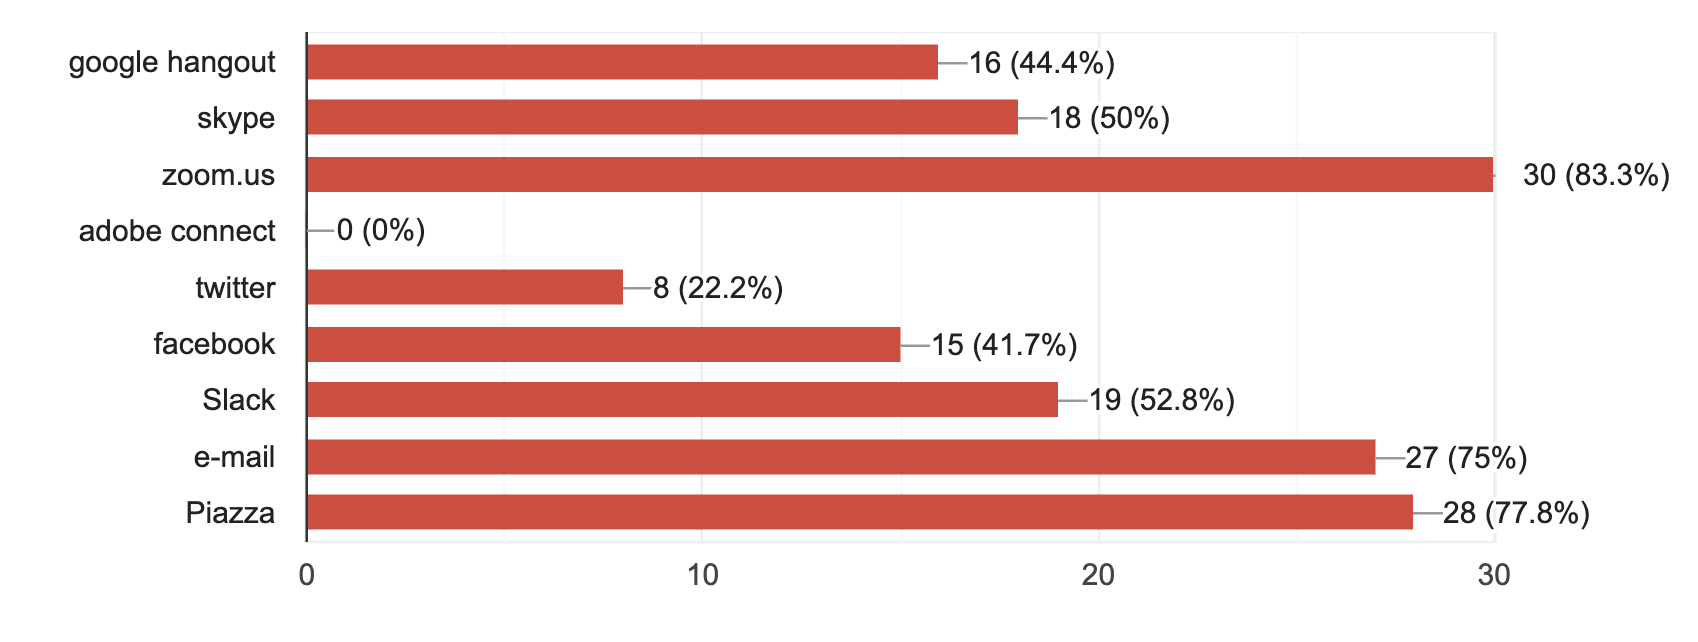
\includegraphics[width=0.9\columnwidth]{images/technologies.png}

\end{figure}


\section{Filling Educational Gaps Technology Knowledge}

Although our course has a small number of requirements, such as knowing a programming language (preferably Python). We asked all of our students, and other than one student, all of them took at least one-semester programming before entering this class. However, we found over the years that the knowledge of {\em real} programming experience by those learning a programming language in the first semester decreases. This is largely motivated by the use of jupyter notebooks in many classes taught at the university level. This goes hand in hand with the teaching of object-oriented programming being taught only at the end of the semester.

Thus it is possible to pass a programming class with a good grade without even knowing the concepts of classes or writing programs outside the jupyter notebook framework. It also does not typically include teaching students advanced tools such as linters that may be built into Python IDE's such as PyCharm. Hence these students are deprived of the more advanced software engineering concepts that the previous generation of students had no issue with.

To emphasize this point, we have conducted a survey in our ongoing class.

We found that 94\% of the students have used Python in the past.  50\% of the students say that Python is their strongest language, followed by Java with 19\% and C\# and R with 8\%. All other languages are below 3\%. While this is would normally be encouraging, we find however, a significant gap in knowledge. We have no students that identify themselves as Python experts, 64\% say they are intermediate, and 36\% say they are novices.

We can back this also up by a more detailed question in which we asked if students are familiar with if conditions, while loops, functions, classes, and parallel programming concepts (see Fig. \ref{fig:python}).

\begin{figure}[htb]
  \caption{Python}\label{fig:python}
  \centering
    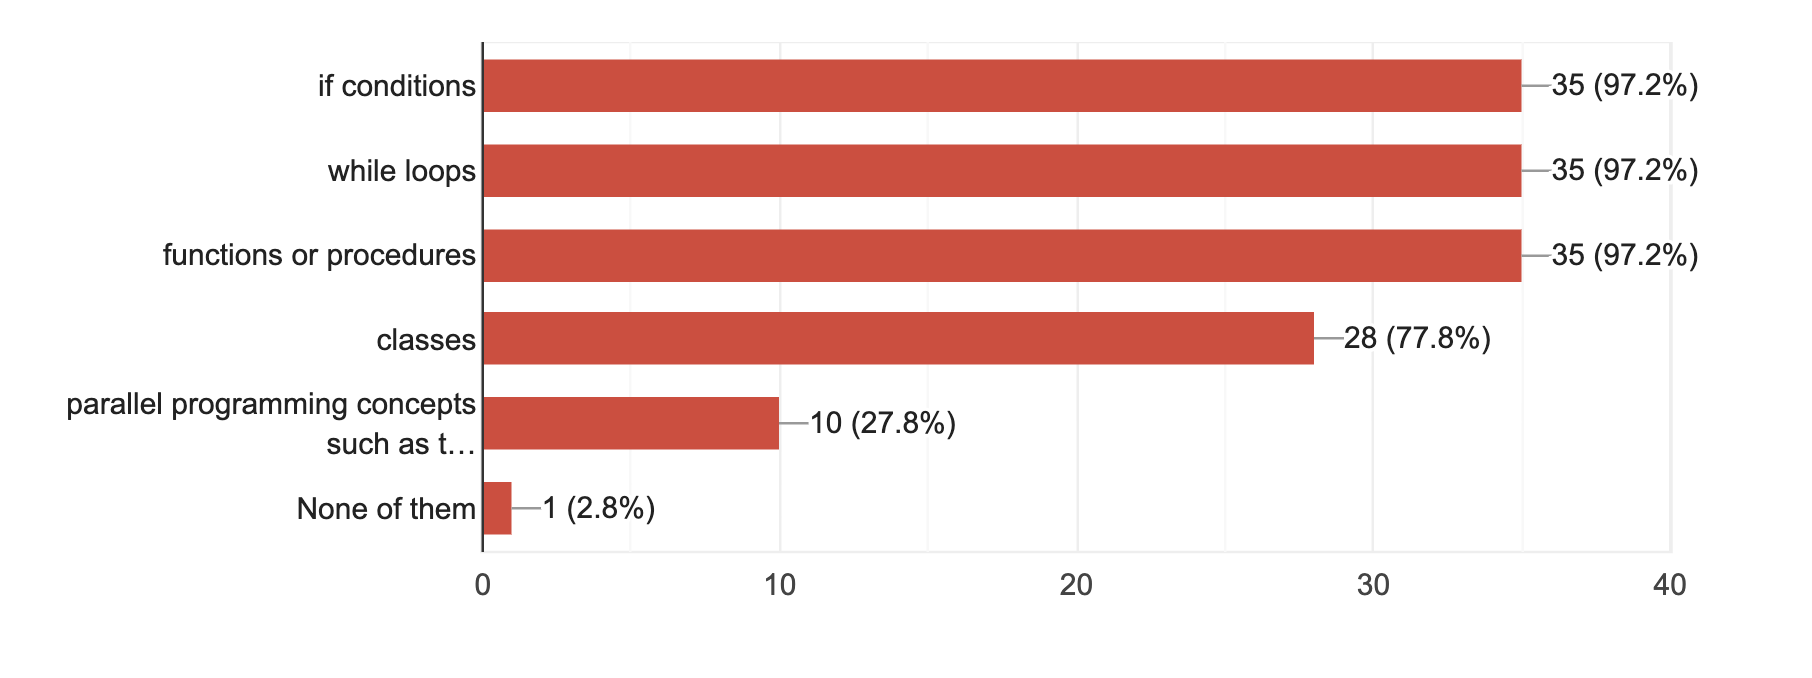
\includegraphics[width=0.9\columnwidth]{images/python.png}

\end{figure}

As we see from this figure almost about 23\% of the students
do not have a background in using classes despite the fact that all but
one student had taken programming classes.

Other basic skills that we need for cloud engineering include shell
scripting and basic knowledge of SSH key management. The knowledge of
SSH is an almost one-to-one reflection of the knowledge of using a
shell terminal (see Fig. \ref{fig:shell} and \ref{fig:ssh})

\begin{figure}[htb]
  \caption{Shell}\label{fig:shell}
  \centering
    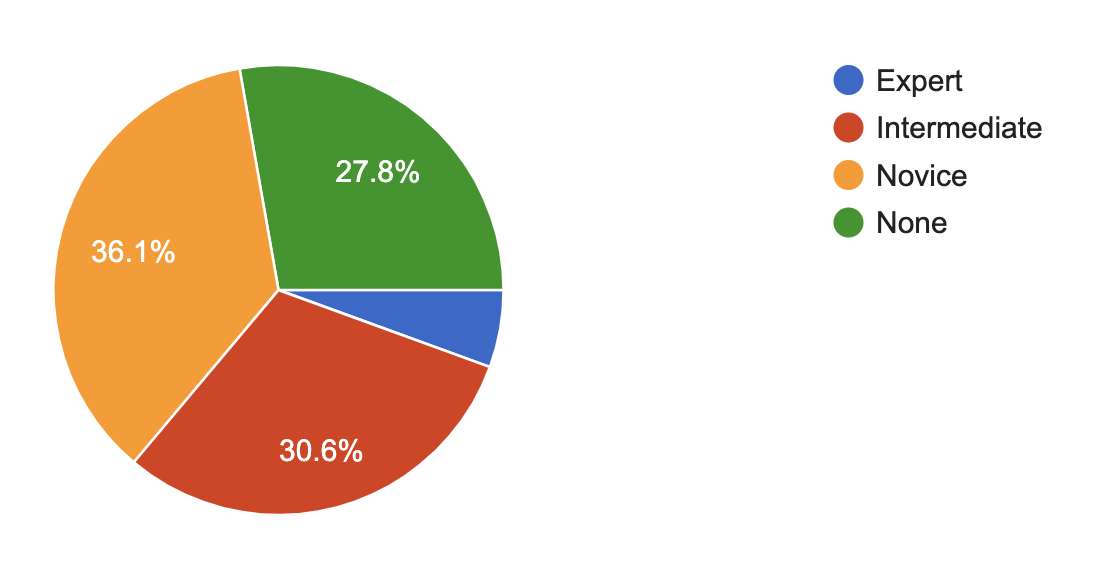
\includegraphics[width=0.9\columnwidth]{images/shell-script.png}

\end{figure}

\begin{figure}[htb]
  \caption{SSH}\label{fig:ssh}
  \centering
    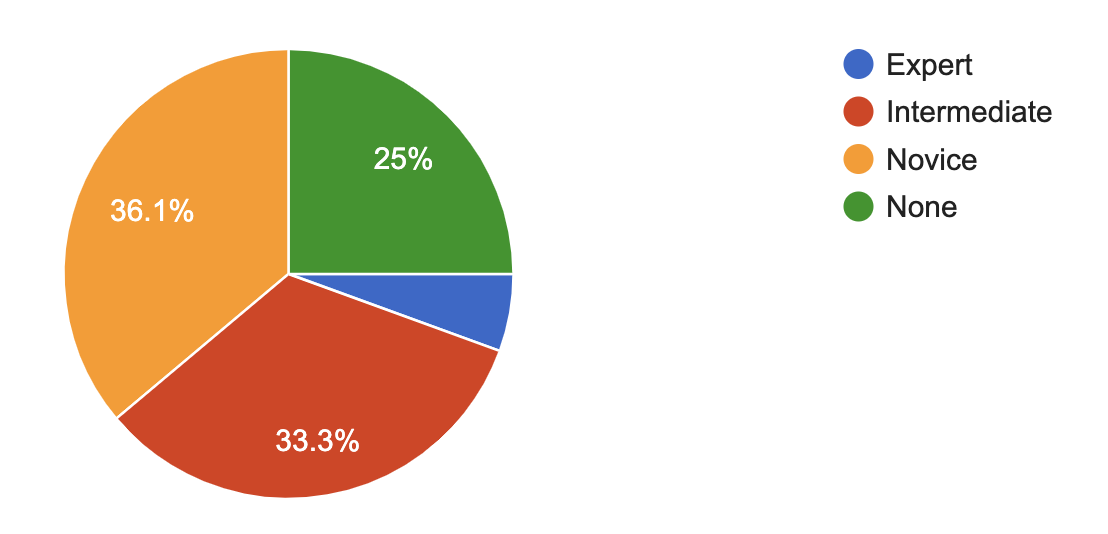
\includegraphics[width=0.9\columnwidth]{images/ssh.png}

\end{figure}

Taking this into account, we need to teach as part of the cloud class
obviously these concepts (e.g., object-oriented programming to
support large codes, shell scripting, ssh, and also advanced IDE's
such as pycharm). Naturally, this takes away time for cloud-related
topics, but it is necessary to be able to conduct complex engineering
tasks that go beyond just toy examples as are addressed in the class
project. To address these issues, we integrate them into our weekly labs
and introduce them as soon as they are needed.


\section{Filling the Gap of Organizational Knowledge}

While in our first classes (some years ago) we left it up to the
students to conduct the Labs on their own without checking we quickly
realized that this resulted in that they are not done at all by most
students. While questioning the students we found out that they spend
all their time on classes that regularly assign weekly homework. Thus
we switched back our class model to also assign homework. However we
have still refrained from introducing tests. After the introduction of
graded lab assignments, we saw a drastic improvement in-class
participation and also less needed help for projects as all our
assignments prepare the students for the project.

The biggest issue we have at this time is that our principle termed.

{\em R2D1 = Read twice and do once}

is not followed by many students. Instead, we often see

{\em R0D0 = Read not and do not succeed}


We have taken extra time out and
observed how students work during the Labs and identified that some
students do not read the material carefully but just jump to our
examples and copy-paste them into their terminals and execute
them. When they missed a requirement to be installed on their
computers that are documented they do not go back and fix their
computers.
Furthermore, we observed that when pointers to external
documentation is provided, such as installing software on Windows, the
remarks on how to enable such software are not read or not understood.
We recently had such a  case as we needed in python to compile the
cryptographic libraries in Windows. The error was clearly presented in the log
messages, but the students' dod not conduct a proper search on google
where a clear solution was posted. Only after the instructor helped
to organize a response with the students, this was addressed. What we
learned out of this is that students do not copy-paste the errors into
a google search to get self-help. Thus this class is not only about
what we teach the students a technical aspect that we present but
also teaches the students what to do when they run into an issue.
In summary, we deal with the issues of
(a) students ar use to immediate regards when clicking on a button in
the Web, while glancing and not comprehending the information
presented 
(b) students are used from other classes that the duration of solving
an issue may be minutes instead of hours
(c) students can not schedule long-lasting assignments and focus
on week-to-week assignments rather than focussing on more important
more significant problem-solving activities.
We believe that through our emphasize on the project while augmenting
it with a week to week assignments we help the organizational skills of
this student generation.

\section{Filling the Gap of Hardware and OS Knowledge}

Although this class can be taken with only a minimal set of hardware
as all resources can be obtained in the cloud. The minimum would be a
Raspberry PI which cost with SD Card, cable, and power supply between
\$50-100 (under the assumption you have a TV or monitor), e.g., the cost
of a textbook. The setup of this is easy and well
documented. However, most students will use their own Laptops or
Desktop computers and rightly expect that some of the work can be done
locally on the computers. This includes things such as simulating a
cloud environment for virtual machines and containers. Although we
originally only supported Linux and macOS we have recently put more
effort in also supporting Windows 10 due to its frequent use in the
student population (see Fig. \ref{fig:os}). As Windows Home does not support
containers or Hyper-V at this time, we typical are helping students
in the first three weeks to transition their machine to use Windows 10
EDU or PRO. However the biggest hurdle we face at this time is that
when measuring the memory consumption done on such a development
computer is more than 8GB, however, 50\% of the students only have  8GB
main memory, thus their work will either be slowed down or not
possible on their machines. This is especially disappointing for those
students that just purchased a machine and found many online reports
that 8GB is enough for a computer. This is no longer true. The good
news is that in case students run into resource limitations, they can
naturally use the cloud, and instead of running containers and VMs on
their local machines, they can interface with them in the cloud.

We also have as already pointed output effort into place to teach
students on how to install the newest version of Python on their
computers which in the case of Windows is  a bit more involved
as it also includes the deployment of the Visual C++ build tools due
too many advanced python libraries not available as pre-compiled wheels
(e.g., cryptographic libraries).

\begin{figure}[htb]
  \caption{Operating System}\label{fig:os}
  \centering
    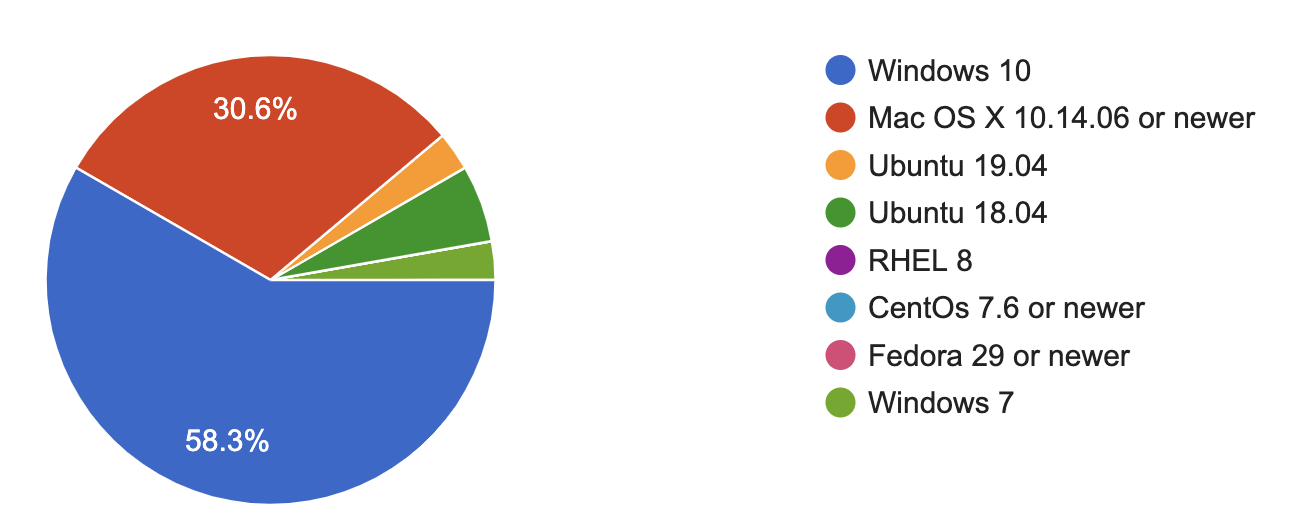
\includegraphics[width=0.9\columnwidth]{images/os.png}

\end{figure}



\begin{figure}[htb]
  \caption{Computer Memory}\label{fig:computer-memory}
  \centering
    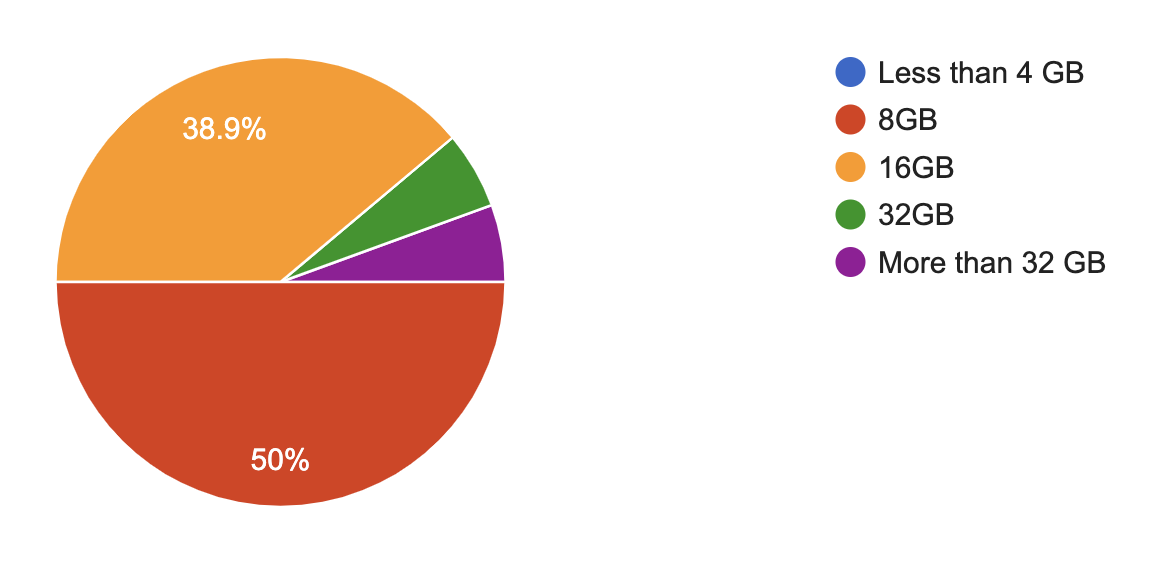
\includegraphics[width=0.9\columnwidth]{images/computer.png}

\end{figure}






\section{Multi-Cloud Engineering}

One of our biggest successes was to integrate our cloudmesh toolkit
into the class that allows us to interface with clouds through a very
simple but sophisticated command line interface. We use cloudmesh to
teach the students various aspects of cloud engineering as listed in
the introduction of this paper.

As a user cloudmesh is extremely simple and allows one to manage, for
example, VMs on different clouds in a similar
matter. Fig. \ref{fig:cloudmesh-multi} shows, for example, that we can
switch booting a VM easily from one cloud to another. Thus even
inexperienced students can comprehend this concept while not having to
initially learn all the different tools or GUIs to manage the various
clouds.

\begin{figure}[htb]

\caption{Cloudmesh usage to start VMs on various clouds}\label{fig:cloudmesh-multi}

\begin{verbatim}
cms set cloud=aws
cms vm boot

cms set cloud=azure
cms vm boot
\end{verbatim}

  \end{figure}

This is made possible by introducing for each cloud an abstract
Provider and integrate it into a sophisticated command shell based on
standard python technologies. Configurable defaults determine which OS
is used for the VM, and which sizes and flavors are used. The
credentials are included in a configuration file (that can be
encrypted) so the need for authentication is minimized. The further
development of cloudmesh can be chosen as a project or cloudmesh can
simply be used to manage virtual machines. Many students have
contributed to make cloudmesh a usable product, but at the same time, it
can be used as a teaching tool.

The Architecture for managing to compute resources via cloudmesh is
depicted in Fig. \ref{fig:cloudmesh-arch}. However, cloudmesh has many
more features, including storage management, virtual directory
management, cost selection.




\begin{figure}[htb]
  \caption{Cloudmesh architecture for compute management}\label{fig:cloudmesh-arch}
  \centering
    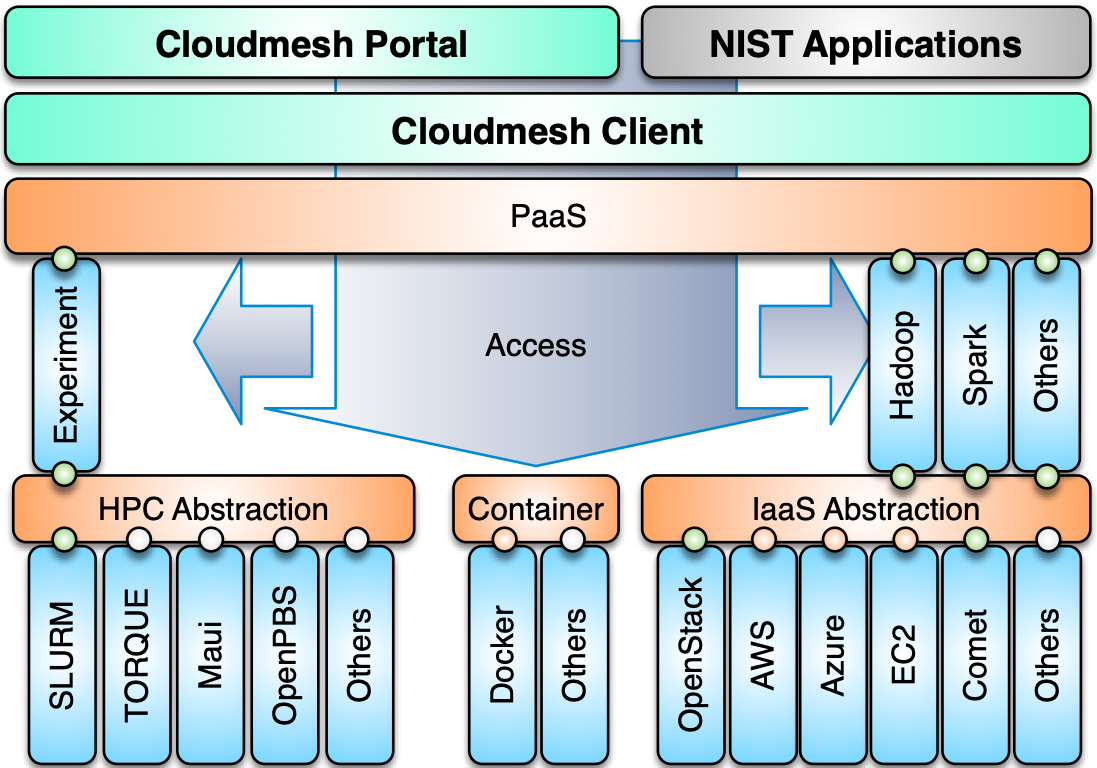
\includegraphics[width=0.9\columnwidth]{images/cloudmesh-arch.png}

\end{figure}


\section{Cloud Resources and Services}

To conduct this class, we are using mostly the free tiers offered by
the main cloud providers. Additionally, we are using the OpenStack KVM 
Cloud offered by Chameleon cloud. We found that beyond these needs, no
other cloud resources are needed at this time. We are developing
however as part of this class within a student project a 100 node
Raspberry PI cluster that will be used to run Kubernetes, Hadoop, and Spark.
Although we have our own research clusters that can also fulfill these
needs, the Raspberry Pi cluster offers the students full access to the
resource. We can configure the cluster in multiple ways by integrating
them in a big cluster or splitting them up in smaller clusters of 5
nodes each. This allows the students to gain access to administrative
tools and services that would otherwise not be accessible to them
within the university setting. Those with enough memory can use their
own laptops to simulate a number of cloud resources through virtual
machines or containers. Also, tools to deploy VMs,  Kubernetes, Hadoop, Spark
and other clusters are available to use the students machine if
resources allow. At one point students in our class are force to
benchmark their project on two different cloud providers.

\section{Customizing Educational Content}

The development of educational material is conducted in three areas (1) component development, (2) enabling technologies,  and (3) outreach activities. We list the activities for each of the areas next.

\subsection{Educational Component Development}

This area contains the development of course material. For the purpose
of this paper, we limit our discussion on the creation of course material
for the courses Engineering Cloud Computing,  Big Data Applications,
Intelligent Systems Engineering for Undergraduates and Graduate
Students. As part of this effort, we developed major new components for
Big Data Applications while integrating new applications and modules
introducing the students to deep learning. The latter was added this
academic year. For the course material relating to Intelligent Systems
Engineering for Undergraduates, we created a mix between cloud
computing and machine learning while leveraging the material that we
also developed for the other two courses.

We have packaged course material with over 52K lines of teaching
material, with 275K words and 1.9M characters, which are freely
available for anyone to reuse. In our book format, these are over 2000
pages. Material from this collection was used in four different
courses.

From this content, we selected numerous chapters and included them in
topical books:

\begin{itemize}
\item  Introduction to Cloud Computing \cite{las20book-cloudeng}
  
\item   Introduction to Python for Cloud Computing \cite{las20book-python}
  
\item  Introduction to Linux \cite{las20book-linux}
  
\item  Introduction to Git

\item Scientific writing with markdown  \cite{las20book-markdown}

\item Cloud Technology Reviews \cite{las20book-tech}

\item Big Data \cite{las20book-bigdata}
  
\end{itemize}


\subsection{Enabling technologies}

One of the issues we face while customizing educational material for
courses and individual students are that there is no tool that
conveniently and easily allows the generation of content contributed
by many course developers in a distributed manner without spending
days and weeks of integrating such content.

However, this kind of
the process is well understood in software development while leveraging
community-driven code repositories.



We evaluated online tools used at
Indiana University to distribute course content including {\em CANVAS}
and {\em EdX} for the automated upload of course content developed by
the community.


First, Neither \emph{CANVAS} nor \emph{OpenEdX} allows the pragmatic
offline development of course material with easy to use standard tools
and then importing the content. We verified this with both platforms. In
the case of \emph{OpenEdX,} we also verified that an open-source tool to
import \emph{LaTeX} is not supported by \emph{OpenEdX}. While
experimenting with it, major limitations were uncovered such as lack of
features, lack of documentation, and bugs, thus making it not suitable
for use.

Second, In \emph{OpenEdX} and \emph{Canvas} content must be developed in
the platform itself through GUI's that are slow and are best suited for
those developing traditional course material that does not allow the
adaptation of individual course adaptation for students.

Third, due to the lack of an import feature for external developed
material, using any existing course management tool results in a
``vendor'' lock-in. This naturally is undesirable as we strive to make
the content of the modules available to everyone regardless if they are
\emph{OpenEdX}, \emph{Canvas}, or are part of another learning content
management system.

Fourth, existing tools to create books such as \emph{LaTeX} and
\emph{Sphinx} have disadvantages due to their focus on a single document
as part of a relatively complex build process when organizing large
diverse content as we do. Hence, customization for individual students
becomes not a matter of minutes, but potentially hours, which is not
acceptable.

Fifth, we had to adapt the course material so far every year due to the
change of technologies while we were teaching the courses. Having the
material in repositories managed in \emph{GitHub} not only allows the
teachers to contribute, but we found that students from Generation Z
were quick to help in updating the material showcasing that we can
benefit from those students in the class that are tech-savvy. The
content could be updated quickly.

Due to these limitations, we are developing a tool called
\emph{\textbf{cyberaide bookmanager}} \cite{pypi-bookmanager}, that
can easily generate custom educational material for students based on
their educational requirements. The material can be distributed on
\emph{GitHub}. To ease the installation of the tool, we have released a
version to the public on \emph{GitHub} and \emph{PyPI}. Based on
community feedback, we not only allow content to be distributed in
\emph{GitHub} but enhanced the tool to include files that can be
managed on the local file system.  Furthermore, we have showcased that
the tool can be used to integrate course material written in different
formats, including \emph{LaTeX}, restructured text, and
\emph{Org-mode}. The tool is using \emph{pandoc}, which supports many
other formats. Next, we list a number of selected features of the \emph{bookmanager}:

\begin{enumerate}
\item  allows easily to combine course material from
  different authors distributed on \emph{GitHub},
  
\item creation of customised table of content using a special YAML
  format we defined allowing the integration of variable substitutions,
  
\item integration of bibliographies,
    
\item automated image downloading from remote content
  repositories,
  
\itme support of various output formats including ePub and PDF, and 

\item platform compatibility due to containerized distribution.
  
\end{enumerate}

\subsection{Outreach Activities and Impact}

Over the last year, we conducted a number of outreach activities.
This included the usage and individualization of content for students
participating as part of REU at Indiana University. For these students,
supervising graduate students developed an individualized curriculum
based on their educational gaps. This included lessons from
\emph{Python}, \emph{Linux}, deep learning, and data processing. The
content was augmented for each student by faculty mentors.
\emph{\textbf{All participating undergraduate students were
minorities.}} In addition, we supported the multi-week effort of the ``Science Gateway
Coding Institute'' at Elizabeth City State University, a
\emph{\textbf{minority-serving institution}} with course material and
teaching support. We prepared material for our next major event is Fall 2019, jointly with
the \emph{nanoBIO} project. We will offer this material with
nanoengineering and bioengineering to a visiting group of about
\emph{\textbf{20 undergraduates from Minority Serving Institutions.}}

However, we believe our biggest achievement is that more than 2000
pages of educational material cast in online books are available to the
entire community for free. Moreover, through the bookmanager that we
developed, custom material can be created by teachers as well as
students taking this class. Student directories, including projects, are
available in GitHub. We currently have where we have 187 repositories
and a total of 172 participants. Furthermore, we have as part of
cloudmesh 95 repositories and 41 participants.

\subsection{NIST Big Data Reference Architecture}

One other outstanding achievement of this work is that results from
this class cast as projects have been integrated into the Nist Big Data
Reference Architecture Working Group. Cloudmesh can be considered as a
reference architecture for selected services that NIST introduces in
tits documents validating the approach. Thus students that participate
in this class have the opportunity to contribute to NIST
\cite{nist-bigdata,nist-vol8} directly.

\section{Conclusion}

We have successfully implemented a cloud computing curriculum that is
available for free and can be reused by educators. Furthermore, we
provide a tool that allows the custom generation of this content
based on selected chapters for educators, as well as students taking
using this material. Thus it is possible not only to generate a {\em
  standard} course applicable to all students, but a {\em
  individualized} custom generated course material based on students'
background and interests. The courses we teach are project-oriented
and allow through the reuse of cloudmesh multi-cloud experiences to be
easily integrated into the class.  Over 2000 pages of educational
material are available that spawn a wide variety of
topics. Collaboration to integrate additional content is
welcome. Please contact \verb|laszewski@gmal.com}.


\section*{Acknowledgment}

This project is in part supported by the NSF Award #1829704
CyberTraining: CIC: CyberTraining for Students and Technologies from
Generation Z. We like to thank the many students that have taken the
classes taught by Gregor von Laszewski and Geoffrey C. Fox  at Indiana
University residential and online program.


\bibliographystyle{./bibliography/IEEEtran}

\bibliography{../../laszewski/hugo/vonLaszewski.bib,../../laszewski/hugo/vonLaszewski-new.bib}

\end{document}


\section{courses}

UUUUUUUUUU


\begin{table*}[htb]
\centering
\caption{TableName}

\begin{tabular}{|p{6cm}|p{10cm}||}
\hline
Task & Comment  \\ \hline
A. Building Training Modules \\ \hline
A.1. Infrastructure for Building Training Modules \\ \hline
Github approach & Documented the GitHub approach we used and improved over the first year of the proposal.  \\ \hline
Bookmanager & Developed a tool to build custom curricula from Markdown hosted in GitHub content. Content can be distributed in various GitHub repositories.   \\ \hline
*  bookmanager to epub & Implemented the feature to create the selected course material as epub.  \\ \hline
*  bookmanager to pdf & Implemented the feature to create the selected course material as epub.  \\ \hline
*  bookmanager import & Demonstrated importing of content written in other formats than Markdown.  \\ \hline
Hosting course material on GitHub & Github has been used to host the course material. The course material content can be written locally or with the help of the GitHub UI in Markdown.   \\ \hline
The transition from LaTeX to Markdown & All content was converted from LaTeX to markdown including the introduction of labels and cross-references. This included reducing the duplication of management and content.  We removed about 60000 lines of duplicated content and management framework scripts. At this time we have \~52K lines of teaching material, with \~275K words and \~1.9M characters all in markdown.   \\ \hline
Evaluation of commodity communication tools for classes & We evaluated Canvas, Slack, and Piazza for class communication. We identified that Piazza is the best tool for us due to its ability to integrate students into the class solution, followed by Slack which is best used in small teams. We recommend others to use either one of these technologies.    \\ \hline
Creation of Course Content in Org-mode & To evaluate the technologies we developed, we tested and verified that content developed by Swany’s team in Org-mode can easily be integrated in bookmanager.   \\ \hline
A.2 Building Course material \\ \hline
Transition to Python 3 & Most all material was transitioned from Python 2.7 to Python 3 as we address the up-coming deprecation of Python 2 in the year 2020   \\ \hline
Cloud Computing, Overview and Introduction & We updated the course material used for 222, 416, 516, 616. Every 6 month the course material has to be improved due to constant development in the field. This includes 16 weeks of lectures for a semester for each class.  \\ \hline
Y1-2 \\ \hline
 \\ \hline
*  Bridging requirements gaps for the class in regards to Python programming & Development of material for the Introduction of Python for Cloud Computing:  We observed that students with  Python background are lacking skills for the cloud engineering classes such as simple object oriented programming, modules, benchmarking, debugging. We will provide a cloud focused introduction to these skills that are demonstrated in the projects.   \\ \hline
 \\ \hline
*  Bridging requirements gaps for the class in regards to document preparation & Development of material on how to use Markdown for project documentation and academic paper writing. This set of material showcases how to use markdown to write documentation for projects or academic papers  \\ \hline
*  Bridging requirements gaps for the class in regards to use of Linux & Linux for Cloud Computing: This set of material introduces Generation Z to command line tools and shells as they are typically not familiar with it due to advanced user interfaces on tablets, phones, and computers that are being taught to students at high school level.   \\ \hline
*  Lecture topics & Development of lectures to introduce Docker   \\ \hline
Development of lectures to introduce Kubernetes   \\ \hline
Development of lectures to introduce REST Services using OpenApi 2.0   \\ \hline
Streaming Data Systems  & Course material for E423 while focussing on Twister2 has been added   \\ \hline
Network Educational Material & Course material was developed as part of a network class taught by Swany   \\ \hline
\end{tabular}
\end{table*}

\begin{table*}
\centering
\caption{TableName}

\begin{tabular}{|p{6cm}|p{10cm}|}
\hline
Task & Comment  \\ \hline
B. Outreach \\ \hline
Science Gateway Coding Institute at Elizabeth City State University  & Workshop successfully completed \\ \hline
REU students hosted at IU used material individually prepared for their tasks & Educational material reused and requirements gathering from Generation Z students   \\ \hline
Broader Impact & We worked together with Elithabeth City University a minority serving institution to distribute our material and reuse the material we developed. We hosted 3 minority students that reused our material   \\ \hline
Engaging Stakeholders & We verified with other departmental stakeholders that the bookmanager is able to integrate other formats such as org mode demonstrating that bookmanager is universally usable.   \\ \hline
We started a discussion with Prof. Sterling about copyrighted material that may be used in other classes as part of already published books. We envision that teaching material can point to such resources and it is easy to integrate with bookmanager.   & started but needs to be completed in Y2 due to Sterling time constraint \\ \hline
Engaging Stakeholders & Coordinating course creation activities with faculty members from the ISE department   \\ \hline
\end{tabular}
\end{table*}

  
